[86 v\textsuperscript{o}]  Liquet igitur ex praecedentibus, quod, si supponatur vitrum  figuram illam habere quam describit \textit{KDB}, circa axem \textit{DI}  rotata, ac semidiametrum circuli \textit{ND} aequari unitati, quod  tum inquam omnes radii in Cylindro ex lineae \textit{AB} circa  axem \textit{DK} circumgyratione orto, contenti, cujus basis  semidiameter aequalis sit \textit{FB}, congregabuntur in producto  axe \textit{DK}, nempe\pend \pstart @@@ G R A F I K @@@% \begin{wrapfigure}{l}{0.4\textwidth}                    
                %\includegraphics[width=0.4\textwidth]{../images/}
                        %\caption{Bildbeschreibung}
                        %\end{wrapfigure}
                        %@ @ @ Dies ist eine Abstandszeile - fuer den Fall, dass mehrere figures hintereinander kommen, ohne dass dazwischen laengerer Text steht. Dies kann zu einer Fahlermeldung fuehren. @ @ @ \\
                     Apparet etiam, si in vitris quorum semidiameter aequatur @@@ G R A F I K @@@% \begin{wrapfigure}{l}{0.4\textwidth}                    
                %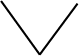
\includegraphics[width=0.4\textwidth]{../images/Zu+einer+Abschrift%2C+Autor+nicht+ermittelt/LH037%2C02_086v/files/100080.png}
                        %\caption{Bildbeschreibung}
                        %\end{wrapfigure}
                        %@ @ @ Dies ist eine Abstandszeile - fuer den Fall, dass mehrere figures hintereinander kommen, ohne dass dazwischen laengerer Text steht. Dies kann zu einer Fahlermeldung fuehren. @ @ @ \\
                     digiti mensurae, sumatur apertura aequalis @@@ G R A F I K @@@% \begin{wrapfigure}{l}{0.4\textwidth}                    
                %\includegraphics[width=0.4\textwidth]{../images/Zu+einer+Abschrift%2C+Autor+nicht+ermittelt/LH037%2C02_086v/files/100082.png}
                        %\caption{Bildbeschreibung}
                        %\end{wrapfigure}
                        %@ @ @ Dies ist eine Abstandszeile - fuer den Fall, dass mehrere figures hintereinander kommen, ohne dass dazwischen laengerer Text steht. Dies kann zu einer Fahlermeldung fuehren. @ @ @ \\
                     quartae partis  digiti, hoc est @@@ G R A F I K @@@% \begin{wrapfigure}{l}{0.4\textwidth}                    
                %\includegraphics[width=0.4\textwidth]{../images/Zu+einer+Abschrift%2C+Autor+nicht+ermittelt/LH037%2C02_086v/files/100086.png}
                        %\caption{Bildbeschreibung}
                        %\end{wrapfigure}
                        %@ @ @ Dies ist eine Abstandszeile - fuer den Fall, dass mehrere figures hintereinander kommen, ohne dass dazwischen laengerer Text steht. Dies kann zu einer Fahlermeldung fuehren. @ @ @ \\
                     pro diametro basis praedicti Cylindri  radiorum (quae longitudo major est semisse semidiametri circuli \textit{NDB}, cujus figuram vitrum induit:) quod tum semidiameter  foci minor erit quam @@@ G R A F I K @@@% \begin{wrapfigure}{l}{0.4\textwidth}                    
                %\includegraphics[width=0.4\textwidth]{../images/Zu+einer+Abschrift%2C+Autor+nicht+ermittelt/LH037%2C02_086v/files/100096.png}
                        %\caption{Bildbeschreibung}
                        %\end{wrapfigure}
                        %@ @ @ Dies ist eine Abstandszeile - fuer den Fall, dass mehrere figures hintereinander kommen, ohne dass dazwischen laengerer Text steht. Dies kann zu einer Fahlermeldung fuehren. @ @ @ \\
                     quartae partis digiti. Unde  constat, focum ipsum pro puncto mechanico\protect\index{Sachverzeichnis}{punctum!mechanicum} tantum habendum 